\documentclass[10pt,oneside,a4paper]{report}
\usepackage{setspace}
\doublespacing
\usepackage[left=1.5in, right=1in, top=1in, bottom=1in]{geometry}
\usepackage{graphicx} %TO include graphics in document
\usepackage{amssymb}
\usepackage{algorithm}% http://ctan.org/pkg/algorithms
\usepackage{algpseudocode}% http://ctan.org/pkg/algorithmicx
\usepackage{cite}
\usepackage{url}

\author{Arpit Gawande}
\title{DDoS Detection and Defense Using Learning Tool}
\date{\today}
\begin{document}

\begin{abstract}
Distributed Denial of Service (DDoS) attacks are common these days\cite{ddosattacknews}. So it is evident that current industry solutions such as completely relying on Internet Service Provider(ISP) or setting up own DDoS infrastructure are not sufficient in detecting and mitigating DDoS attacks, hence consistent research is needed. Most of the current industry solutions involve setting up centralized expensive hardware system which can analyze the network data packets\footnote{We would call it \lq{packet}\rq or \lq{packets}\rq in rest of the paper}\cite{networkdatapacket} for probable DDoS attacks. Also each organization or ISP has different systems which are not compatible with other ISP's. In this paper we are going to discuss another a way to detect and mitigate DDoS attack using machine learning tools.
\end{abstract}

\chapter{Existing Systems}

Distributed Denial of Service (DDoS) attack is the way to jam host network or its resources with large number of data packets, so that host become disabled to serve. The real challenge in detecting and defending DDoS attack is because of its dynamic nature. The source\footnote{It is a system/device on the Internet which has an IP address and which is involved in DDoS attack} is not a single node or system on the Internet but many, and often distributed over the Internet. Also the source of the packet is often spoofed, which makes more harder to know the actual Internet address of system from where attack is originated because they hide original attack source. On top of that, many times the source itself is not aware that it is compromised and has been used as bot\cite{bot} by attacker.

Detecting and mitigating attack at the destination is not very useful as because destination may know that the attack is happening but to stop it happening it will have to block all the incoming traffic including the legitimate traffic, because source address can not be reliable way to know the attack source. To avoid this, firm which provide the networking devices have come up with solutions.

Many of the solutions available in the market or the research that was done is to collect network traffic flow\cite{networkTrafficFlow} (we would call it just flow) samples at routers(gateways) and feed/send it on the central system to analyze. Central system is a hardware and software infrastructure which is capable of processing and analyzing large flow information.

Some of the major protocols which are widely used for flow collection and analysis are, Internet Protocol Flow Information Export (IPFIX) protocol created by Internet Engineering Task Force (IETF), Ciscos NetFlow\cite{cisconetflow} and Sflow(Sampled flow)\cite{sflow}. These protocols have defined standard way to export flow information from router and similar devices. All these flow monitoring protocols gather information and send the consolidated flow information to the centralized server where user can login and do analyses for different purpose such as Security Monitoring, Bandwidth monitoring, Resource Management, Traffic Analysis, Performance Management. It will have some modules which are specifically used for anomaly/DDoS detection.

E.g. Cisco netflow has flow Exporter, Collector and Analysis modules. Flow exporter is generally router who send flow information to collector module which acts as flow storage. Analysis module then try to find out different patterns in the flow.

These technologies scales well and sufficient to indicate trends in network traffic but they have limitations. 1. They are not cross platform, e.g. Sflow router would not be able to work with Cisco routers. 2. They involve setting up expensive hardware which would act as collector server. 3. In these technologies source address is used for flow analysis but as we know it is not reliable due to IP spoofing in in case of of DDoS attacks.

now we know that router based flow analysis would be useful for anomaly detection but we don't want to set up expensive hardware, we want to have protocol or system which is not compatible with other routers also we want to only rely on destination IP address for flow\footnote{In our paper we would consider flow only in sense of destination address} analysis. So if we could come up with the way by which we could detect anomaly in the traffic at the routers independent of manufacturer, and create a protocol to communicate the attack parameters to allow routers to take decisions then we would be more efficient in detecting and mitigating DDoS attacks.

If we use the learning algorithm at the router and if router could learn the normal behavior of the flow then if there is any anomaly then it will be able to identify it from its previous learning and that change in behavior of the traffic can be communicate to destination network.

With the advance of electronic and the Internet of things, electronic devices are getting equipped with faster processor and fast memories. Router are also not left behind. Only thing that is missing is the storage space. If we use the learning techniques which don't need much storage then we don't have to store the packets instead we would learn from every flow and discard once learning is done. This is necessary because number of entries on the Internet routing table has steadily grown.  Now that the table has passed 500,000 routes\cite{routingtablesize} so storing each and every flow information for these routes could be difficult.\par

\chapter{DDoS Detection and Mitigation}
One of the way to detect the DDoS attack is to check for anomalous behavior in the network traffic. This can be done at different points. Either at the destination server or at the router. Once the attack is detected by observing the behavior of the traffic to mitigate it we would have to block all the packets which are causing the attack. One of the way to identify those packets is by their source address.

\chapter{Network Functioning}
A switch creates a network and router connects networks. A router links computers to the Internet through other routers. Routers are the backbone of the network who helps to forward packet from one point to other point on the Internet. Every packet traveling on Internet has to go through router\cite{swithcrouter}.Router knows where the packet is destine hence it could serve as first point of knowledge about the change in the flow information for a destine network. Each router has interfaces to which hosts or other network are connected. So router is aware to whom it is connected. Router uses protocol to communicate and by that they gather knowledge about other networks or router on the Internet. ICMP\cite{icmp} is one of the most frequently use protocol by routers to communicate.\par

\begin{figure}[H]
  \label{fig:Routers}
  \centering
    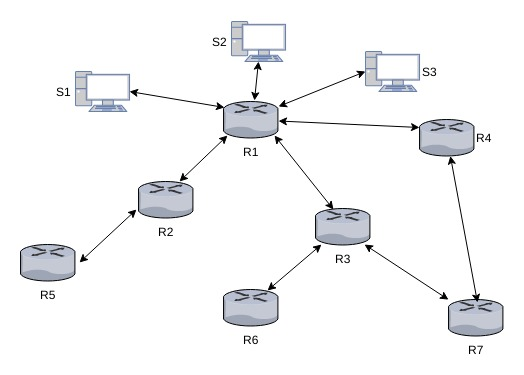
\includegraphics[width=0.80\textwidth]{Routers}
    \caption{Network Example}
\end{figure}


Lets illustrated this using an example. In the above figure we can see that host S1, S2, S3 are connected to router R1. Router R1 is connected to Internet through router R2, R3, R4 , thus every packet that would be reaching to S2 would come from either of these three routers. All three routers are locates at different geographical region. Most of the websites are regional, either county, state or national (If we leave out few global websites) and hence they are mostly accessed from those region it is meant for. E.g. Rutgers University website would be accessed mostly from the eastern region of United States and that too mostly from the New Jersey State or the Philadelphia region. \par
Using traceroute we can find out how many hope away the destination is. Each hope is the router on the Internet. Following is one of the captured traceroute for Rutgers University website.\par
%\vspace{5mm} % vertical space
\begin{figure}[H]
  \label{fig:Traceroute}
  \centering
    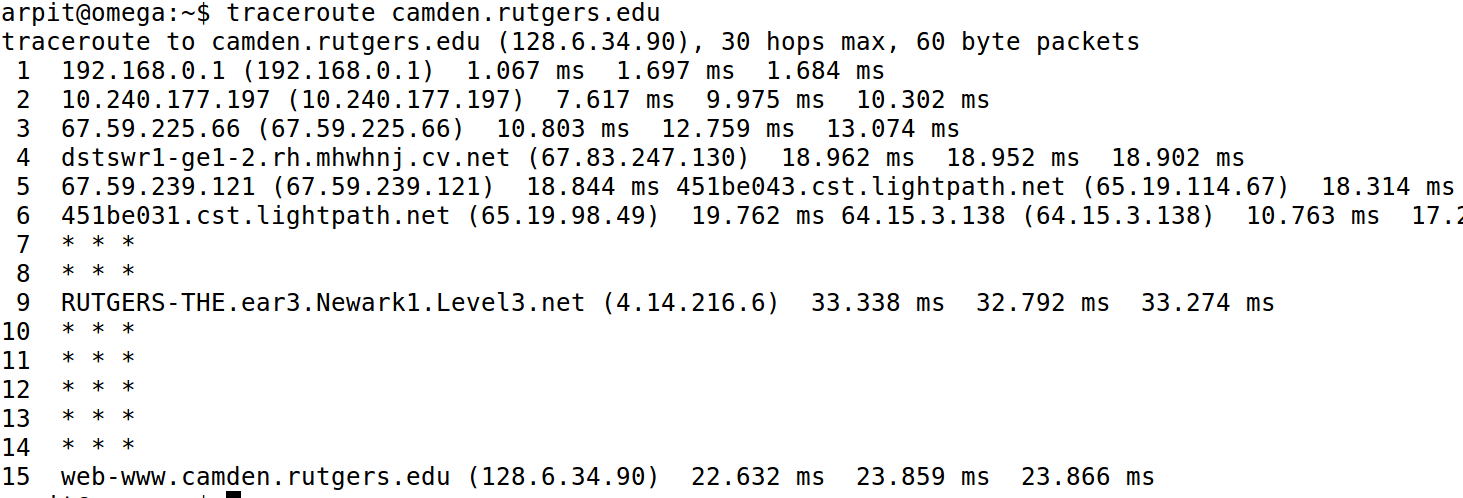
\includegraphics[width=\textwidth]{TraceRoute}
      \caption{Trace Route: All the routers in the path to destination}
\end{figure}


We can see that there are about 14 routers (if we don't consider the home router 192.168.0.1) to reach to the camden.rutgers.edu. This trace route is taken from a location in the New Jersey State.


\chapter{Suggested New Approach}
From figure \ref{fig:Routers} and \ref{fig:Traceroute} we know that routers are located at different geographical locations and also we know that there is pattern in which the particular destination website is getting accessed from the different regions. Some of the service providers such as  GeoIP or Google can find out the location from where the traffic is coming in the network for a given destination, but that is approximate based on the source IP, which in the case of DDoS attack is unreliable information because packet source address are often spoofed. So it could be difficult to know the actual geographical location from which packet has come. Only routers can provide the correct geographical information about the source of the packet.\par

In the normal scenario there would be some definite pattern in which the website is getting accessed from different regions and this pattern can be learned over the time with learning algorithms at the routers. Thus finding this pattern in the flow at the router can form the basis of our analysis. When ever there is deviation from the normal pattern of the flow for a particular destination then that change in pattern as well as the geographical region can be communicated to the destination network. Destination network on receiving that information can decide based on the region and how much is the deviation from the normal to decide whether it want the reporting router to discard or forward the traffic for the destination. This is selective process in which traffic from other routers remain unaffected\par

\begin{figure}[H]
  \centering
    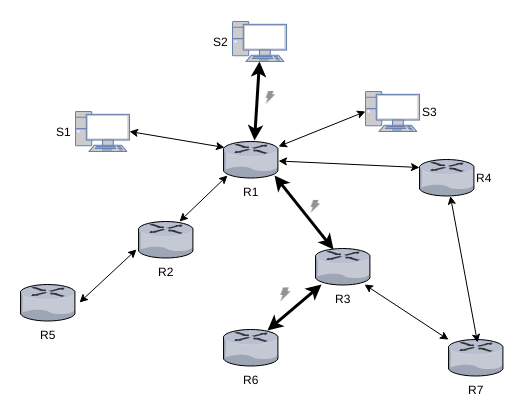
\includegraphics[width=0.90\textwidth]{RouterCommunication}
    \caption{DDoS Attack path}
\end{figure}


In the above figure attack initiated from the region where router R6 is located and from R6 data packets reach to victim from R3 and R1. If we could detect attack at R6 itself then we can discard packets at R6 which are heading towards S2, while traffic from other routers remain unaffected.

To achieve this we would measure the flow during a time window (e.g 300 sec) whose size would be fixed at the beginning.
These time windows can be combined to form a period which is a portion of a day during which traffic is measured. Once we have flow information we can apply learning techniques on each flow iteratively to gain deeper knowledge about normal behavior of the flow.\par

In the proposed system, each router will itself act as a analyzer. Each packet will be analyzed and flow statistic would be created based on the destination IP address. Based on the statistic we would cluster destination IP address using input feature vector. Clustering is the process of examining a collection of “points,” and grouping the points into “clusters” according to some distance measure.The goal is that
points in the same cluster have a small distance from one another, while points in different clusters are at a large distance from one another\cite{clusterning}.

\begin{figure}[H]
  \centering
    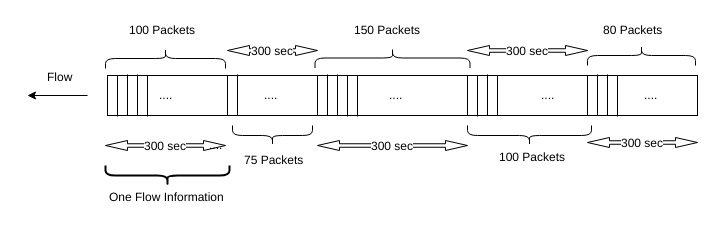
\includegraphics[width=0.90\textwidth]{Data_Flow_Capture}
    \caption{Data Flow Segments}
\end{figure}


Once cluster is learned it would be used as bench mark for all future flow. Router would constantly keep clustering destination IP and if there is deviation in the normal traffic at router for a destination then that would affect the clustering and would cause destination to be placed in different cluster, cluster with more packet frequency. This change in clustering would be reported to destination network, which then decide on regulating the traffic\par

\chapter{Implementation}
Botnet(Network  of bots) plays important role in DDoS attack. Bots are the compromised system controlled by attacker for launching attack. Those can be anywhere on the Internet they are not bounded by geographical boundaries. The major DDoS attacks are the volume based attacks. So for this paper we would be considering only the volume based attack for the simplicity.\par
Wireshark, an open source application, was used for capturing Internet packet. Packets are captured for 5 hr on a single router for the demonstration purpose. Once the packets are captured they are saved as pcapng file which is a Wireshark file format for captured packets. Wireshark capture every detail of the packets but we don't need all of the information, we would only be interested in the IP packets.\par
\begin{figure}[H]
  \centering
    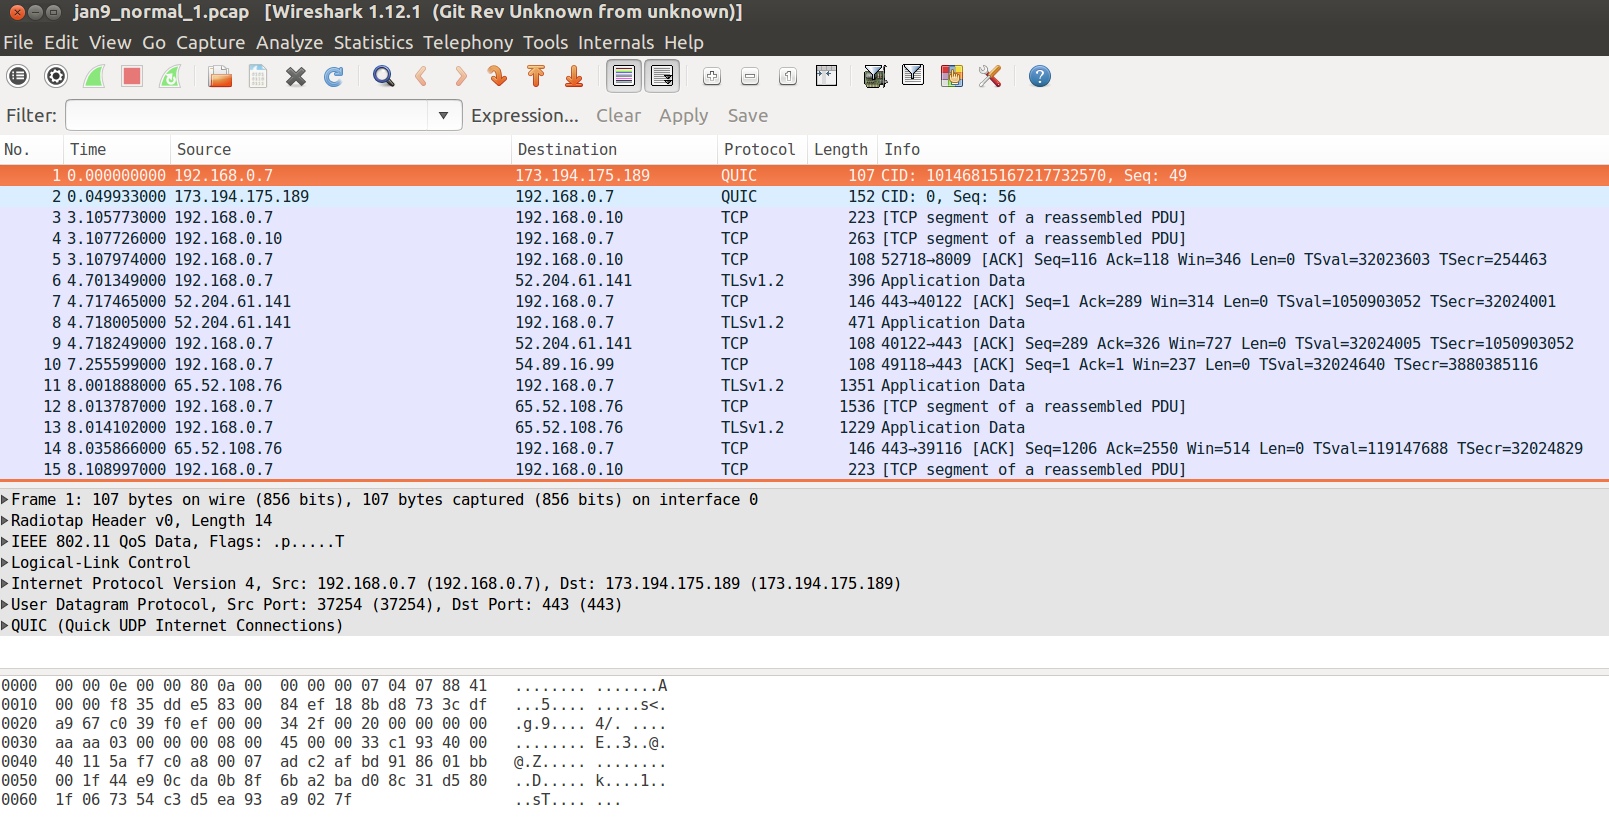
\includegraphics[width=0.90\textwidth]{Wireshark_Tools.png}
    \caption{Wireshark Tool: snippet of captured packets}
\end{figure}


To extract data from the captured packets data extraction program \textit{data\_extraction} is written in Python. Flow is logically treated as IP packets captured over 300 second time and that is considered as one sample flow. Because of of the limited resource each frame is written to the file with time and sample number. Once we have extracted information form all the packets and sampled in different files then we can use them to create feature table. Another program \textit{IP\_clustering} is used for clustering the samples. Our data sample would look like below\par
\begin{figure}[H]
  \centering
    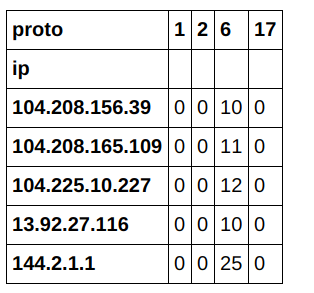
\includegraphics[width=0.50\textwidth]{dataframe.png}
    \caption{Flow Information for given destinations}
\end{figure}


Number in the table represents the frequency of the packet of the particular protocol destine for particular destination. For our clustering algorithm, frequency of the protocol would serve as feature vector. For the sake of simplicity we would be dealing with TCP and UPD flood attacks. Attack is engineered using LOIC (Low Orbit Ion Canon), a free tool which is even used by attackers in the real world. Flow based model is build as it is more reliable and fast because packet analyzing is often difficult due to size and encryption also destination port could not a reliable information in detecting attacks as attacker use different ports.

There are many algorithms which can be used to learn from the data, they can be categorized as Supervised or Unsupervised.

According to Tom Mitchell (1998) A computer program is said to learn from experience E with respect to some task T and some performance measure P, if its performance on T, as measured by P, improves with experience.

Let $f$ be the function which we need to guessed from input vector X = $x^{1}$, $x^{2}$, ..., $x^{m}$ and $h$ be the hypothesis about the function $f$. $h \in H$ and $f \in H$, where $H$ is class of functions. Both $f$ and $h$ can be vectors. We select $h$ based on a
training set, $\Xi$, of $m$ input vector examples. In Supervised leaning we know the values of $f$ for the $m$ samples in the training set $\Xi$. We assume that if we can find a hypothesis, $h$, that closely agrees with $f$ for the members of $\Xi$, then this hypothesis will be a good guess for $f$ when $\Xi$ is large. In Unsupervised learning, we simply have a training set of vectors without function values for them. The problem in this case, typically, is to partition the training set into subsets, $\Xi_1$,  ,$\Xi_R$, in some appropriate way.\cite{clusterning}

Supervised algorithm such as One Class Support Vector Machine(SVM) could be efficient to identify the anomalies in the data but it is very process and memory intensive so they can be used only for the highest cluster IP address. Unsupervised learning algorithms are fast and consume less data so they would be useful for our analysis at router level.

k-means clustering is one of the most efficient algorithm for creating clusters. In k-means, problem is to find set of $k$ points ($k \in \mathbb{N}$) in $\mathbb{R}^d$ $(\mu_{1}, \mu_{2}, ..., \mu_{k})$, called centers, such that mean square distance $(argmin_{k} || x^{i} {-} \mu_{k} ||^{2})$ from each data point from the set of $n$ data points in $d-dimension—l$ space ‚$\mathbb{R}^d$ to its nearest center from $k$ centers is minimum. Lloyd's algorithm is most popular heuristic for k-me—ans clustering.

\chapter{Algorithms}

\begin{algorithm}
\caption{Lloyd's algorithm k-means algorithm}\label{kmeans}
\begin{algorithmic}
\State{$x^{1}$, $x^{2}$, ..., $x^{m}$ is training set, where $x^{i} \in \mathbb{R}^d$, $i = 1,2, .., m$}
\State {Randomly initialize k cluster centroids $\mu_{1}$, $\mu_{2}$, ..., $\mu_{k} \in \mathbb{R}^d$}
\Repeat
  \For{$i\gets 1, m$}
    %\State {$c^{i}$ = index (from 1 to K) of cluster centroid closest to $x^{i}$}
    \State{$c^{i} = argmin_{k} || x^{i} {-} \mu_{k} ||^{2}$}\Comment{Cluster Assignment}
  \EndFor
  \For{$k\gets 1, K$}
    %\State {$\mu_{i}$ = average (mean) of points assigned to cluster k}
    \State{$\mu_{k} = \frac{1}{n} [x^{(k_{1})} + x^{(k_{2})} + ... + x^{(k_{n}})] \in R$}\Comment{Move Centroid}
  \EndFor
\Until convergence
\end{algorithmic}
\end{algorithm}

\begin{algorithm}
\caption{Algorithm for DDoS attack Detection}\label{detectmitigate}
  \begin{algorithmic}[1]
  \State{Divide traffic into minor time window (e.g. 300 sec).}
  \State{Filter data based on the required features.}
  \State{Run Clustering algorithm on the data. (Use elbow method to decide on number of clusters).}
  \State{Find the probability of certain IP lying in a particular cluster.}
  \State{Once the clusters are decided our model is ready.}
  \State{now to test model we would cluster and label each IP and if there is change in the cluster.}
  \State{If No change $\rightarrow$ traffic is normal.}
  \State{If change change $\rightarrow$ traffic not normal.}
  \end{algorithmic}
\end{algorithm}

Once the change in the normal behavior has been reported then router communicate to the destination network. Destination network collect that information to know the source of the attack. This information can be used to know the nature of the attack.

\section{Conclusion}
A novel way to identify and mitigate DDoS attack is discussed in the paper. With the advance of NVF(Network Virtual Functional) it would be easy to push the learning algorithms to the routers and thus making them efficient in detecting the attacks. Also ICMP protocol can be used to communicate location and attack information in between the routers.

\bibliographystyle{unsrt}   % Unsorted order
\bibliography{biblo}       % expects file "biblo.bib"

\end{document}
